\documentclass[1p]{elsarticle_modified}
%\bibliographystyle{elsarticle-num}

%\usepackage[colorlinks]{hyperref}
%\usepackage{abbrmath_seonhwa} %\Abb, \Ascr, \Acal ,\Abf, \Afrak
\usepackage{amsfonts}
\usepackage{amssymb}
\usepackage{amsmath}
\usepackage{amsthm}
\usepackage{scalefnt}
\usepackage{amsbsy}
\usepackage{kotex}
\usepackage{caption}
\usepackage{subfig}
\usepackage{color}
\usepackage{graphicx}
\usepackage{xcolor} %% white, black, red, green, blue, cyan, magenta, yellow
\usepackage{float}
\usepackage{setspace}
\usepackage{hyperref}

\usepackage{tikz}
\usetikzlibrary{arrows}

\usepackage{multirow}
\usepackage{array} % fixed length table
\usepackage{hhline}

%%%%%%%%%%%%%%%%%%%%%
\makeatletter
\renewcommand*\env@matrix[1][\arraystretch]{%
	\edef\arraystretch{#1}%
	\hskip -\arraycolsep
	\let\@ifnextchar\new@ifnextchar
	\array{*\c@MaxMatrixCols c}}
\makeatother %https://tex.stackexchange.com/questions/14071/how-can-i-increase-the-line-spacing-in-a-matrix
%%%%%%%%%%%%%%%

\usepackage[normalem]{ulem}

\newcommand{\msout}[1]{\ifmmode\text{\sout{\ensuremath{#1}}}\else\sout{#1}\fi}
%SOURCE: \msout is \stkout macro in https://tex.stackexchange.com/questions/20609/strikeout-in-math-mode

\newcommand{\cancel}[1]{
	\ifmmode
	{\color{red}\msout{#1}}
	\else
	{\color{red}\sout{#1}}
	\fi
}

\newcommand{\add}[1]{
	{\color{blue}\uwave{#1}}
}

\newcommand{\replace}[2]{
	\ifmmode
	{\color{red}\msout{#1}}{\color{blue}\uwave{#2}}
	\else
	{\color{red}\sout{#1}}{\color{blue}\uwave{#2}}
	\fi
}

\newcommand{\Sol}{\mathcal{S}} %segment
\newcommand{\D}{D} %diagram
\newcommand{\A}{\mathcal{A}} %arc


%%%%%%%%%%%%%%%%%%%%%%%%%%%%%5 test

\def\sl{\operatorname{\textup{SL}}(2,\Cbb)}
\def\psl{\operatorname{\textup{PSL}}(2,\Cbb)}
\def\quan{\mkern 1mu \triangleright \mkern 1mu}

\theoremstyle{definition}
\newtheorem{thm}{Theorem}[section]
\newtheorem{prop}[thm]{Proposition}
\newtheorem{lem}[thm]{Lemma}
\newtheorem{ques}[thm]{Question}
\newtheorem{cor}[thm]{Corollary}
\newtheorem{defn}[thm]{Definition}
\newtheorem{exam}[thm]{Example}
\newtheorem{rmk}[thm]{Remark}
\newtheorem{alg}[thm]{Algorithm}

\newcommand{\I}{\sqrt{-1}}
\begin{document}

%\begin{frontmatter}
%
%\title{Boundary parabolic representations of knots up to 8 crossings}
%
%%% Group authors per affiliation:
%\author{Yunhi Cho} 
%\address{Department of Mathematics, University of Seoul, Seoul, Korea}
%\ead{yhcho@uos.ac.kr}
%
%
%\author{Seonhwa Kim} %\fnref{s_kim}}
%\address{Center for Geometry and Physics, Institute for Basic Science, Pohang, 37673, Korea}
%\ead{ryeona17@ibs.re.kr}
%
%\author{Hyuk Kim}
%\address{Department of Mathematical Sciences, Seoul National University, Seoul 08826, Korea}
%\ead{hyukkim@snu.ac.kr}
%
%\author{Seokbeom Yoon}
%\address{Department of Mathematical Sciences, Seoul National University, Seoul, 08826,  Korea}
%\ead{sbyoon15@snu.ac.kr}
%
%\begin{abstract}
%We find all boundary parabolic representation of knots up to 8 crossings.
%
%\end{abstract}
%\begin{keyword}
%    \MSC[2010] 57M25 
%\end{keyword}
%
%\end{frontmatter}

%\linenumbers
%\tableofcontents
%
\newcommand\colored[1]{\textcolor{white}{\rule[-0.35ex]{0.8em}{1.4ex}}\kern-0.8em\color{red} #1}%
%\newcommand\colored[1]{\textcolor{white}{ #1}\kern-2.17ex	\textcolor{white}{ #1}\kern-1.81ex	\textcolor{white}{ #1}\kern-2.15ex\color{red}#1	}

{\Large $\underline{11a_{255}~(K11a_{255})}$}

\setlength{\tabcolsep}{10pt}
\renewcommand{\arraystretch}{1.6}
\vspace{1cm}\begin{tabular}{m{100pt}>{\centering\arraybackslash}m{274pt}}
\multirow{5}{120pt}{
	\centering
	\includegraphics[width=112pt]{../../../GIT/diagram.site/Diagrams/png/504_11a_255.png}\\
\ \ \ A knot diagram\footnotemark}&
\allowdisplaybreaks
\textbf{Linearized knot diagam} \\
\cline{2-2}
 &
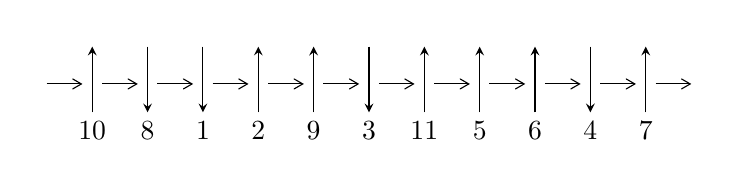
\begin{tikzpicture}[x=20pt, y=17pt]
	% nodes
	\node (C0) at (0, 0) {};
	\node (C1) at (1, 0) {};
	\node (C1U) at (1, +1) {};
	\node (C1D) at (1, -1) {10};

	\node (C2) at (2, 0) {};
	\node (C2U) at (2, +1) {};
	\node (C2D) at (2, -1) {8};

	\node (C3) at (3, 0) {};
	\node (C3U) at (3, +1) {};
	\node (C3D) at (3, -1) {1};

	\node (C4) at (4, 0) {};
	\node (C4U) at (4, +1) {};
	\node (C4D) at (4, -1) {2};

	\node (C5) at (5, 0) {};
	\node (C5U) at (5, +1) {};
	\node (C5D) at (5, -1) {9};

	\node (C6) at (6, 0) {};
	\node (C6U) at (6, +1) {};
	\node (C6D) at (6, -1) {3};

	\node (C7) at (7, 0) {};
	\node (C7U) at (7, +1) {};
	\node (C7D) at (7, -1) {11};

	\node (C8) at (8, 0) {};
	\node (C8U) at (8, +1) {};
	\node (C8D) at (8, -1) {5};

	\node (C9) at (9, 0) {};
	\node (C9U) at (9, +1) {};
	\node (C9D) at (9, -1) {6};

	\node (C10) at (10, 0) {};
	\node (C10U) at (10, +1) {};
	\node (C10D) at (10, -1) {4};

	\node (C11) at (11, 0) {};
	\node (C11U) at (11, +1) {};
	\node (C11D) at (11, -1) {7};
	\node (C12) at (12, 0) {};

	% arrows
	\draw[->,>={angle 60}]
	(C0) edge (C1) (C1) edge (C2) (C2) edge (C3) (C3) edge (C4) (C4) edge (C5) (C5) edge (C6) (C6) edge (C7) (C7) edge (C8) (C8) edge (C9) (C9) edge (C10) (C10) edge (C11) (C11) edge (C12) ;	\draw[->,>=stealth]
	(C1D) edge (C1U) (C2U) edge (C2D) (C3U) edge (C3D) (C4D) edge (C4U) (C5D) edge (C5U) (C6U) edge (C6D) (C7D) edge (C7U) (C8D) edge (C8U) (C9D) edge (C9U) (C10U) edge (C10D) (C11D) edge (C11U) ;
	\end{tikzpicture} \\
\hhline{~~} \\& 
\textbf{Solving Sequence} \\ \cline{2-2} 
 &
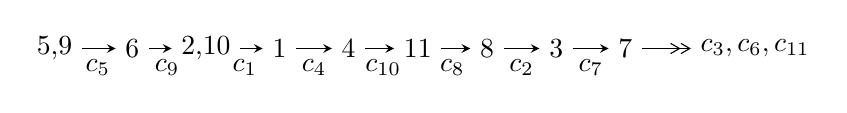
\begin{tikzpicture}[x=25pt, y=7pt]
	% node
	\node (A0) at (-1/8, 0) {5,9};
	\node (A1) at (1, 0) {6};
	\node (A2) at (33/16, 0) {2,10};
	\node (A3) at (25/8, 0) {1};
	\node (A4) at (33/8, 0) {4};
	\node (A5) at (41/8, 0) {11};
	\node (A6) at (49/8, 0) {8};
	\node (A7) at (57/8, 0) {3};
	\node (A8) at (65/8, 0) {7};
	\node (C1) at (1/2, -1) {$c_{5}$};
	\node (C2) at (3/2, -1) {$c_{9}$};
	\node (C3) at (21/8, -1) {$c_{1}$};
	\node (C4) at (29/8, -1) {$c_{4}$};
	\node (C5) at (37/8, -1) {$c_{10}$};
	\node (C6) at (45/8, -1) {$c_{8}$};
	\node (C7) at (53/8, -1) {$c_{2}$};
	\node (C8) at (61/8, -1) {$c_{7}$};
	\node (A9) at (10, 0) {$c_{3},c_{6},c_{11}$};

	% edge
	\draw[->,>=stealth]	
	(A0) edge (A1) (A1) edge (A2) (A2) edge (A3) (A3) edge (A4) (A4) edge (A5) (A5) edge (A6) (A6) edge (A7) (A7) edge (A8) ;
	\draw[->>,>={angle 60}]	
	(A8) edge (A9);
\end{tikzpicture} \\ 

\end{tabular} \\

\footnotetext{
The image of knot diagram is generated by the software ``\textbf{Draw programme}" developed by Andrew Bartholomew(\url{http://www.layer8.co.uk/maths/draw/index.htm\#Running-draw}), where we modified some parts for our purpose(\url{https://github.com/CATsTAILs/LinksPainter}).
}\phantom \\ \newline 
\centering \textbf{Ideals for irreducible components\footnotemark of $X_{\text{par}}$} 
 
\begin{align*}
I^u_{1}&=\langle 
1.80659\times10^{126} u^{87}+6.62202\times10^{126} u^{86}+\cdots+8.45954\times10^{125} b-6.83566\times10^{124},\\
\phantom{I^u_{1}}&\phantom{= \langle  }6.92943\times10^{125} u^{87}+2.71684\times10^{125} u^{86}+\cdots+8.45954\times10^{125} a+3.63682\times10^{126},\;u^{88}+3 u^{87}+\cdots+12 u-1\rangle \\
I^u_{2}&=\langle 
6 u^{16}-5 u^{15}+\cdots+b+9,\;-4 u^{16}+3 u^{15}+\cdots+a-3,\;u^{17}-2 u^{16}+\cdots+2 u-1\rangle \\
\\
\end{align*}
\raggedright * 2 irreducible components of $\dim_{\mathbb{C}}=0$, with total 105 representations.\\
\footnotetext{All coefficients of polynomials are rational numbers. But the coefficients are sometimes approximated in decimal forms when there is not enough margin.}
\newpage
\renewcommand{\arraystretch}{1}
\centering \section*{I. $I^u_{1}= \langle 1.81\times10^{126} u^{87}+6.62\times10^{126} u^{86}+\cdots+8.46\times10^{125} b-6.84\times10^{124},\;6.93\times10^{125} u^{87}+2.72\times10^{125} u^{86}+\cdots+8.46\times10^{125} a+3.64\times10^{126},\;u^{88}+3 u^{87}+\cdots+12 u-1 \rangle$}
\flushleft \textbf{(i) Arc colorings}\\
\begin{tabular}{m{7pt} m{180pt} m{7pt} m{180pt} }
\flushright $a_{5}=$&$\begin{pmatrix}1\\0\end{pmatrix}$ \\
\flushright $a_{9}=$&$\begin{pmatrix}0\\u\end{pmatrix}$ \\
\flushright $a_{6}=$&$\begin{pmatrix}1\\- u^2\end{pmatrix}$ \\
\flushright $a_{2}=$&$\begin{pmatrix}-0.819125 u^{87}-0.321157 u^{86}+\cdots+16.0138 u-4.29907\\-2.13556 u^{87}-7.82787 u^{86}+\cdots+22.9711 u+0.0808042\end{pmatrix}$ \\
\flushright $a_{10}=$&$\begin{pmatrix}u\\- u^3+u\end{pmatrix}$ \\
\flushright $a_{1}=$&$\begin{pmatrix}-0.129180 u^{87}+0.672098 u^{86}+\cdots+3.50283 u-3.01968\\-2.64974 u^{87}-8.65151 u^{86}+\cdots-3.14880 u+2.43678\end{pmatrix}$ \\
\flushright $a_{4}=$&$\begin{pmatrix}-2.08531 u^{87}-5.49795 u^{86}+\cdots+25.3255 u-0.354318\\-1.84736 u^{87}-5.50308 u^{86}+\cdots+87.1798 u-7.04699\end{pmatrix}$ \\
\flushright $a_{11}=$&$\begin{pmatrix}-1.83766 u^{87}-6.94809 u^{86}+\cdots-62.8333 u+11.5382\\-0.322083 u^{87}-1.44486 u^{86}+\cdots+69.6894 u-6.79609\end{pmatrix}$ \\
\flushright $a_{8}=$&$\begin{pmatrix}- u\\u\end{pmatrix}$ \\
\flushright $a_{3}=$&$\begin{pmatrix}-0.332721 u^{87}-0.302475 u^{86}+\cdots+27.5489 u-5.01410\\-2.62197 u^{87}-7.84655 u^{86}+\cdots+11.4361 u+0.795836\end{pmatrix}$ \\
\flushright $a_{7}=$&$\begin{pmatrix}0.00418543 u^{87}-0.339575 u^{86}+\cdots+87.8936 u-8.51572\\-0.524156 u^{87}+1.20963 u^{86}+\cdots+25.6387 u-2.61072\end{pmatrix}$\\ \flushright $a_{7}=$&$\begin{pmatrix}0.00418543 u^{87}-0.339575 u^{86}+\cdots+87.8936 u-8.51572\\-0.524156 u^{87}+1.20963 u^{86}+\cdots+25.6387 u-2.61072\end{pmatrix}$\\&\end{tabular}
\flushleft \textbf{(ii) Obstruction class $= -1$}\\~\\
\flushleft \textbf{(iii) Cusp Shapes $= -1.27706 u^{87}-1.69690 u^{86}+\cdots+382.685 u-26.5055$}\\~\\
\newpage\renewcommand{\arraystretch}{1}
\flushleft \textbf{(iv) u-Polynomials at the component}\newline \\
\begin{tabular}{m{50pt}|m{274pt}}
Crossings & \hspace{64pt}u-Polynomials at each crossing \\
\hline $$\begin{aligned}c_{1}\end{aligned}$$&$\begin{aligned}
&u^{88}+9 u^{87}+\cdots-24 u-1
\end{aligned}$\\
\hline $$\begin{aligned}c_{2}\end{aligned}$$&$\begin{aligned}
&u^{88}- u^{87}+\cdots+1530 u-73
\end{aligned}$\\
\hline $$\begin{aligned}c_{3}\end{aligned}$$&$\begin{aligned}
&u^{88}+2 u^{87}+\cdots+1392 u+133
\end{aligned}$\\
\hline $$\begin{aligned}c_{4}\end{aligned}$$&$\begin{aligned}
&u^{88}-3 u^{87}+\cdots+6998 u+2363
\end{aligned}$\\
\hline $$\begin{aligned}c_{5},c_{8},c_{9}\end{aligned}$$&$\begin{aligned}
&u^{88}-3 u^{87}+\cdots-12 u-1
\end{aligned}$\\
\hline $$\begin{aligned}c_{6}\end{aligned}$$&$\begin{aligned}
&u^{88}- u^{87}+\cdots+9888 u-1216
\end{aligned}$\\
\hline $$\begin{aligned}c_{7},c_{11}\end{aligned}$$&$\begin{aligned}
&u^{88}+26 u^{86}+\cdots+35 u-19
\end{aligned}$\\
\hline $$\begin{aligned}c_{10}\end{aligned}$$&$\begin{aligned}
&u^{88}+5 u^{87}+\cdots+32 u-1
\end{aligned}$\\
\hline
\end{tabular}\\~\\
\newpage\renewcommand{\arraystretch}{1}
\flushleft \textbf{(v) Riley Polynomials at the component}\newline \\
\begin{tabular}{m{50pt}|m{274pt}}
Crossings & \hspace{64pt}Riley Polynomials at each crossing \\
\hline $$\begin{aligned}c_{1}\end{aligned}$$&$\begin{aligned}
&y^{88}-15 y^{87}+\cdots+48 y+1
\end{aligned}$\\
\hline $$\begin{aligned}c_{2}\end{aligned}$$&$\begin{aligned}
&y^{88}+17 y^{87}+\cdots+439816 y+5329
\end{aligned}$\\
\hline $$\begin{aligned}c_{3}\end{aligned}$$&$\begin{aligned}
&y^{88}-16 y^{87}+\cdots-1724598 y+17689
\end{aligned}$\\
\hline $$\begin{aligned}c_{4}\end{aligned}$$&$\begin{aligned}
&y^{88}-23 y^{87}+\cdots-69312708 y+5583769
\end{aligned}$\\
\hline $$\begin{aligned}c_{5},c_{8},c_{9}\end{aligned}$$&$\begin{aligned}
&y^{88}-87 y^{87}+\cdots+6 y+1
\end{aligned}$\\
\hline $$\begin{aligned}c_{6}\end{aligned}$$&$\begin{aligned}
&y^{88}-7 y^{87}+\cdots-41894912 y+1478656
\end{aligned}$\\
\hline $$\begin{aligned}c_{7},c_{11}\end{aligned}$$&$\begin{aligned}
&y^{88}+52 y^{87}+\cdots+8009 y+361
\end{aligned}$\\
\hline $$\begin{aligned}c_{10}\end{aligned}$$&$\begin{aligned}
&y^{88}-9 y^{87}+\cdots-42 y+1
\end{aligned}$\\
\hline
\end{tabular}\\~\\
\newpage\flushleft \textbf{(vi) Complex Volumes and Cusp Shapes}
$$\begin{array}{c|c|c}  
\text{Solutions to }I^u_{1}& \I (\text{vol} + \sqrt{-1}CS) & \text{Cusp shape}\\
 \hline 
\begin{aligned}
u &= -0.461471 + 0.841006 I \\
a &= \phantom{-}0.528338 + 0.458503 I \\
b &= -1.067760 + 0.659062 I\end{aligned}
 & \phantom{-}0.94916 - 7.07982 I & \phantom{-0.000000 } 0 \\ \hline\begin{aligned}
u &= -0.461471 - 0.841006 I \\
a &= \phantom{-}0.528338 - 0.458503 I \\
b &= -1.067760 - 0.659062 I\end{aligned}
 & \phantom{-}0.94916 + 7.07982 I & \phantom{-0.000000 } 0 \\ \hline\begin{aligned}
u &= \phantom{-}0.461917 + 0.839983 I \\
a &= \phantom{-}0.521449 - 0.561797 I \\
b &= -1.15881 - 0.86775 I\end{aligned}
 & -2.63728 + 13.13360 I & \phantom{-0.000000 } 0 \\ \hline\begin{aligned}
u &= \phantom{-}0.461917 - 0.839983 I \\
a &= \phantom{-}0.521449 + 0.561797 I \\
b &= -1.15881 + 0.86775 I\end{aligned}
 & -2.63728 - 13.13360 I & \phantom{-0.000000 } 0 \\ \hline\begin{aligned}
u &= \phantom{-}0.716320 + 0.759777 I \\
a &= -0.096496 - 0.698922 I \\
b &= -0.910905 + 0.530988 I\end{aligned}
 & -1.90928 - 7.75289 I & \phantom{-0.000000 } 0 \\ \hline\begin{aligned}
u &= \phantom{-}0.716320 - 0.759777 I \\
a &= -0.096496 + 0.698922 I \\
b &= -0.910905 - 0.530988 I\end{aligned}
 & -1.90928 + 7.75289 I & \phantom{-0.000000 } 0 \\ \hline\begin{aligned}
u &= -0.747640 + 0.738917 I \\
a &= \phantom{-}0.185794 + 0.644451 I \\
b &= -0.800040 - 0.321449 I\end{aligned}
 & \phantom{-}1.75411 + 1.70043 I & \phantom{-0.000000 } 0 \\ \hline\begin{aligned}
u &= -0.747640 - 0.738917 I \\
a &= \phantom{-}0.185794 - 0.644451 I \\
b &= -0.800040 + 0.321449 I\end{aligned}
 & \phantom{-}1.75411 - 1.70043 I & \phantom{-0.000000 } 0 \\ \hline\begin{aligned}
u &= \phantom{-}0.462797 + 0.784939 I \\
a &= \phantom{-}0.713999 - 0.375007 I \\
b &= -0.575391 - 0.639112 I\end{aligned}
 & -4.87171 + 1.98745 I & \phantom{-0.000000 } 0 \\ \hline\begin{aligned}
u &= \phantom{-}0.462797 - 0.784939 I \\
a &= \phantom{-}0.713999 + 0.375007 I \\
b &= -0.575391 + 0.639112 I\end{aligned}
 & -4.87171 - 1.98745 I & \phantom{-0.000000 } 0\\
 \hline 
 \end{array}$$\newpage$$\begin{array}{c|c|c}  
\text{Solutions to }I^u_{1}& \I (\text{vol} + \sqrt{-1}CS) & \text{Cusp shape}\\
 \hline 
\begin{aligned}
u &= \phantom{-}0.661971 + 0.926980 I \\
a &= -0.0387633 + 0.1080350 I \\
b &= \phantom{-}0.248682 + 0.443728 I\end{aligned}
 & -4.12384 + 3.33457 I & \phantom{-0.000000 } 0 \\ \hline\begin{aligned}
u &= \phantom{-}0.661971 - 0.926980 I \\
a &= -0.0387633 - 0.1080350 I \\
b &= \phantom{-}0.248682 - 0.443728 I\end{aligned}
 & -4.12384 - 3.33457 I & \phantom{-0.000000 } 0 \\ \hline\begin{aligned}
u &= -0.708244 + 0.478843 I \\
a &= -0.296258 - 0.177834 I \\
b &= \phantom{-}0.853123 - 0.895770 I\end{aligned}
 & -0.49529 - 4.30405 I & \phantom{-0.000000 } 0 \\ \hline\begin{aligned}
u &= -0.708244 - 0.478843 I \\
a &= -0.296258 + 0.177834 I \\
b &= \phantom{-}0.853123 + 0.895770 I\end{aligned}
 & -0.49529 + 4.30405 I & \phantom{-0.000000 } 0 \\ \hline\begin{aligned}
u &= \phantom{-}0.830448 + 0.798387 I \\
a &= \phantom{-}0.0650164 - 0.0284208 I \\
b &= -0.131884 + 0.335388 I\end{aligned}
 & -4.10019 + 3.25868 I & \phantom{-0.000000 } 0 \\ \hline\begin{aligned}
u &= \phantom{-}0.830448 - 0.798387 I \\
a &= \phantom{-}0.0650164 + 0.0284208 I \\
b &= -0.131884 - 0.335388 I\end{aligned}
 & -4.10019 - 3.25868 I & \phantom{-0.000000 } 0 \\ \hline\begin{aligned}
u &= \phantom{-}1.210430 + 0.168812 I \\
a &= \phantom{-}0.657008 - 0.139362 I \\
b &= \phantom{-}0.238030 + 0.541756 I\end{aligned}
 & \phantom{-}1.12675 + 3.01989 I & \phantom{-0.000000 } 0 \\ \hline\begin{aligned}
u &= \phantom{-}1.210430 - 0.168812 I \\
a &= \phantom{-}0.657008 + 0.139362 I \\
b &= \phantom{-}0.238030 - 0.541756 I\end{aligned}
 & \phantom{-}1.12675 - 3.01989 I & \phantom{-0.000000 } 0 \\ \hline\begin{aligned}
u &= -1.242660 + 0.064543 I \\
a &= \phantom{-}0.356767 + 0.064742 I \\
b &= \phantom{-}0.259039 + 1.176710 I\end{aligned}
 & -0.78403 + 3.10651 I & \phantom{-0.000000 } 0 \\ \hline\begin{aligned}
u &= -1.242660 - 0.064543 I \\
a &= \phantom{-}0.356767 - 0.064742 I \\
b &= \phantom{-}0.259039 - 1.176710 I\end{aligned}
 & -0.78403 - 3.10651 I & \phantom{-0.000000 } 0\\
 \hline 
 \end{array}$$\newpage$$\begin{array}{c|c|c}  
\text{Solutions to }I^u_{1}& \I (\text{vol} + \sqrt{-1}CS) & \text{Cusp shape}\\
 \hline 
\begin{aligned}
u &= -0.752023 + 0.025277 I \\
a &= \phantom{-}1.248130 - 0.539713 I \\
b &= -0.373499 + 0.173438 I\end{aligned}
 & \phantom{-}1.43199 - 0.10841 I & \phantom{-}9.03393 - 1.67726 I \\ \hline\begin{aligned}
u &= -0.752023 - 0.025277 I \\
a &= \phantom{-}1.248130 + 0.539713 I \\
b &= -0.373499 - 0.173438 I\end{aligned}
 & \phantom{-}1.43199 + 0.10841 I & \phantom{-}9.03393 + 1.67726 I \\ \hline\begin{aligned}
u &= \phantom{-}1.265790 + 0.009736 I \\
a &= \phantom{-}2.61060 + 0.86684 I \\
b &= -1.59560 - 0.66566 I\end{aligned}
 & -0.88817 - 4.15422 I & \phantom{-0.000000 } 0 \\ \hline\begin{aligned}
u &= \phantom{-}1.265790 - 0.009736 I \\
a &= \phantom{-}2.61060 - 0.86684 I \\
b &= -1.59560 + 0.66566 I\end{aligned}
 & -0.88817 + 4.15422 I & \phantom{-0.000000 } 0 \\ \hline\begin{aligned}
u &= -0.083085 + 0.724734 I \\
a &= \phantom{-}1.158860 + 0.095466 I \\
b &= \phantom{-}0.431630 + 0.250640 I\end{aligned}
 & -2.63186 + 0.30603 I & -4.47610 + 0.84684 I \\ \hline\begin{aligned}
u &= -0.083085 - 0.724734 I \\
a &= \phantom{-}1.158860 - 0.095466 I \\
b &= \phantom{-}0.431630 - 0.250640 I\end{aligned}
 & -2.63186 - 0.30603 I & -4.47610 - 0.84684 I \\ \hline\begin{aligned}
u &= -0.406517 + 0.596845 I \\
a &= -0.134387 - 0.848786 I \\
b &= \phantom{-}1.080960 - 0.597180 I\end{aligned}
 & \phantom{-}1.08733 - 1.99106 I & \phantom{-}6.09235 + 1.36477 I \\ \hline\begin{aligned}
u &= -0.406517 - 0.596845 I \\
a &= -0.134387 + 0.848786 I \\
b &= \phantom{-}1.080960 + 0.597180 I\end{aligned}
 & \phantom{-}1.08733 + 1.99106 I & \phantom{-}6.09235 - 1.36477 I \\ \hline\begin{aligned}
u &= -1.28104\phantom{ +0.000000I} \\
a &= \phantom{-}1.92302\phantom{ +0.000000I} \\
b &= -1.09485\phantom{ +0.000000I}\end{aligned}
 & \phantom{-}2.27296\phantom{ +0.000000I} & \phantom{-0.000000 } 0 \\ \hline\begin{aligned}
u &= -1.279570 + 0.203713 I \\
a &= \phantom{-}1.06056 + 0.94410 I \\
b &= -0.895929 - 0.812012 I\end{aligned}
 & \phantom{-}1.161850 - 0.746665 I & \phantom{-0.000000 } 0\\
 \hline 
 \end{array}$$\newpage$$\begin{array}{c|c|c}  
\text{Solutions to }I^u_{1}& \I (\text{vol} + \sqrt{-1}CS) & \text{Cusp shape}\\
 \hline 
\begin{aligned}
u &= -1.279570 - 0.203713 I \\
a &= \phantom{-}1.06056 - 0.94410 I \\
b &= -0.895929 + 0.812012 I\end{aligned}
 & \phantom{-}1.161850 + 0.746665 I & \phantom{-0.000000 } 0 \\ \hline\begin{aligned}
u &= -0.322097 + 0.620023 I \\
a &= \phantom{-}0.315508 - 0.621708 I \\
b &= \phantom{-}0.946527 - 0.186707 I\end{aligned}
 & \phantom{-}0.94922 - 1.67367 I & \phantom{-}6.07995 + 4.98191 I \\ \hline\begin{aligned}
u &= -0.322097 - 0.620023 I \\
a &= \phantom{-}0.315508 + 0.621708 I \\
b &= \phantom{-}0.946527 + 0.186707 I\end{aligned}
 & \phantom{-}0.94922 + 1.67367 I & \phantom{-}6.07995 - 4.98191 I \\ \hline\begin{aligned}
u &= \phantom{-}0.332971 + 0.562296 I \\
a &= -0.68132 + 1.26827 I \\
b &= \phantom{-}1.05330 + 1.02301 I\end{aligned}
 & \phantom{-}0.17356 + 4.65502 I & \phantom{-}2.68890 - 10.30148 I \\ \hline\begin{aligned}
u &= \phantom{-}0.332971 - 0.562296 I \\
a &= -0.68132 - 1.26827 I \\
b &= \phantom{-}1.05330 - 1.02301 I\end{aligned}
 & \phantom{-}0.17356 - 4.65502 I & \phantom{-}2.68890 + 10.30148 I \\ \hline\begin{aligned}
u &= \phantom{-}1.349230 + 0.081552 I \\
a &= -0.072511 - 1.110690 I \\
b &= -0.00272 + 1.71935 I\end{aligned}
 & \phantom{-}3.28529 + 3.22075 I & \phantom{-0.000000 } 0 \\ \hline\begin{aligned}
u &= \phantom{-}1.349230 - 0.081552 I \\
a &= -0.072511 + 1.110690 I \\
b &= -0.00272 - 1.71935 I\end{aligned}
 & \phantom{-}3.28529 - 3.22075 I & \phantom{-0.000000 } 0 \\ \hline\begin{aligned}
u &= \phantom{-}1.352360 + 0.095803 I \\
a &= -2.37770 - 0.49924 I \\
b &= \phantom{-}0.479377 + 0.433404 I\end{aligned}
 & \phantom{-}0.04809 + 6.65339 I & \phantom{-0.000000 } 0 \\ \hline\begin{aligned}
u &= \phantom{-}1.352360 - 0.095803 I \\
a &= -2.37770 + 0.49924 I \\
b &= \phantom{-}0.479377 - 0.433404 I\end{aligned}
 & \phantom{-}0.04809 - 6.65339 I & \phantom{-0.000000 } 0 \\ \hline\begin{aligned}
u &= \phantom{-}0.511484 + 0.381620 I \\
a &= \phantom{-}1.12929 - 2.15831 I \\
b &= -0.702835 - 0.184361 I\end{aligned}
 & -1.90539 + 5.37165 I & \phantom{-}4.99409 - 10.30612 I\\
 \hline 
 \end{array}$$\newpage$$\begin{array}{c|c|c}  
\text{Solutions to }I^u_{1}& \I (\text{vol} + \sqrt{-1}CS) & \text{Cusp shape}\\
 \hline 
\begin{aligned}
u &= \phantom{-}0.511484 - 0.381620 I \\
a &= \phantom{-}1.12929 + 2.15831 I \\
b &= -0.702835 + 0.184361 I\end{aligned}
 & -1.90539 - 5.37165 I & \phantom{-}4.99409 + 10.30612 I \\ \hline\begin{aligned}
u &= \phantom{-}0.164196 + 0.612873 I \\
a &= \phantom{-}0.375315 + 0.193004 I \\
b &= -1.129360 + 0.356278 I\end{aligned}
 & -3.27941 - 2.28675 I & -3.82551 + 1.37856 I \\ \hline\begin{aligned}
u &= \phantom{-}0.164196 - 0.612873 I \\
a &= \phantom{-}0.375315 - 0.193004 I \\
b &= -1.129360 - 0.356278 I\end{aligned}
 & -3.27941 + 2.28675 I & -3.82551 - 1.37856 I \\ \hline\begin{aligned}
u &= -1.382080 + 0.113573 I \\
a &= \phantom{-}0.23821 + 1.80685 I \\
b &= -0.56801 - 2.23826 I\end{aligned}
 & \phantom{-}0.79244 - 7.21107 I & \phantom{-0.000000 } 0 \\ \hline\begin{aligned}
u &= -1.382080 - 0.113573 I \\
a &= \phantom{-}0.23821 - 1.80685 I \\
b &= -0.56801 + 2.23826 I\end{aligned}
 & \phantom{-}0.79244 + 7.21107 I & \phantom{-0.000000 } 0 \\ \hline\begin{aligned}
u &= \phantom{-}1.391480 + 0.005846 I \\
a &= -1.256520 + 0.038074 I \\
b &= \phantom{-}0.961160 - 1.030150 I\end{aligned}
 & \phantom{-}4.81925 - 2.14563 I & \phantom{-0.000000 } 0 \\ \hline\begin{aligned}
u &= \phantom{-}1.391480 - 0.005846 I \\
a &= -1.256520 - 0.038074 I \\
b &= \phantom{-}0.961160 + 1.030150 I\end{aligned}
 & \phantom{-}4.81925 + 2.14563 I & \phantom{-0.000000 } 0 \\ \hline\begin{aligned}
u &= -1.367910 + 0.282397 I \\
a &= -0.943677 - 0.996974 I \\
b &= \phantom{-}1.134880 + 0.127270 I\end{aligned}
 & \phantom{-}5.06894 - 1.03566 I & \phantom{-0.000000 } 0 \\ \hline\begin{aligned}
u &= -1.367910 - 0.282397 I \\
a &= -0.943677 + 0.996974 I \\
b &= \phantom{-}1.134880 - 0.127270 I\end{aligned}
 & \phantom{-}5.06894 + 1.03566 I & \phantom{-0.000000 } 0 \\ \hline\begin{aligned}
u &= -1.411040 + 0.057384 I \\
a &= -1.90492 + 0.51638 I \\
b &= \phantom{-}1.046140 + 0.137041 I\end{aligned}
 & \phantom{-}5.63533 - 2.97696 I & \phantom{-0.000000 } 0\\
 \hline 
 \end{array}$$\newpage$$\begin{array}{c|c|c}  
\text{Solutions to }I^u_{1}& \I (\text{vol} + \sqrt{-1}CS) & \text{Cusp shape}\\
 \hline 
\begin{aligned}
u &= -1.411040 - 0.057384 I \\
a &= -1.90492 - 0.51638 I \\
b &= \phantom{-}1.046140 - 0.137041 I\end{aligned}
 & \phantom{-}5.63533 + 2.97696 I & \phantom{-0.000000 } 0 \\ \hline\begin{aligned}
u &= -1.43441 + 0.20928 I \\
a &= -2.21776 + 0.04987 I \\
b &= \phantom{-}1.41019 - 1.20573 I\end{aligned}
 & \phantom{-}5.87411 - 7.49299 I & \phantom{-0.000000 } 0 \\ \hline\begin{aligned}
u &= -1.43441 - 0.20928 I \\
a &= -2.21776 - 0.04987 I \\
b &= \phantom{-}1.41019 + 1.20573 I\end{aligned}
 & \phantom{-}5.87411 + 7.49299 I & \phantom{-0.000000 } 0 \\ \hline\begin{aligned}
u &= \phantom{-}1.45850 + 0.22546 I \\
a &= -1.93667 + 0.23400 I \\
b &= \phantom{-}1.62738 + 0.88334 I\end{aligned}
 & \phantom{-}7.10229 + 5.03178 I & \phantom{-0.000000 } 0 \\ \hline\begin{aligned}
u &= \phantom{-}1.45850 - 0.22546 I \\
a &= -1.93667 - 0.23400 I \\
b &= \phantom{-}1.62738 - 0.88334 I\end{aligned}
 & \phantom{-}7.10229 - 5.03178 I & \phantom{-0.000000 } 0 \\ \hline\begin{aligned}
u &= \phantom{-}1.46091 + 0.26784 I \\
a &= -1.41901 + 0.35326 I \\
b &= \phantom{-}1.32346 + 0.58187 I\end{aligned}
 & \phantom{-}6.71196 + 5.09265 I & \phantom{-0.000000 } 0 \\ \hline\begin{aligned}
u &= \phantom{-}1.46091 - 0.26784 I \\
a &= -1.41901 - 0.35326 I \\
b &= \phantom{-}1.32346 - 0.58187 I\end{aligned}
 & \phantom{-}6.71196 - 5.09265 I & \phantom{-0.000000 } 0 \\ \hline\begin{aligned}
u &= \phantom{-}0.463199 + 0.202675 I \\
a &= -0.925640 - 0.568827 I \\
b &= \phantom{-}0.895298 + 0.761077 I\end{aligned}
 & \phantom{-}0.58871 + 2.37016 I & \phantom{-}4.17793 + 0.20978 I \\ \hline\begin{aligned}
u &= \phantom{-}0.463199 - 0.202675 I \\
a &= -0.925640 + 0.568827 I \\
b &= \phantom{-}0.895298 - 0.761077 I\end{aligned}
 & \phantom{-}0.58871 - 2.37016 I & \phantom{-}4.17793 - 0.20978 I \\ \hline\begin{aligned}
u &= -1.49052 + 0.12670 I \\
a &= -2.00668 + 0.39222 I \\
b &= \phantom{-}1.61947 - 0.73656 I\end{aligned}
 & \phantom{-}7.08647 - 3.90826 I & \phantom{-0.000000 } 0\\
 \hline 
 \end{array}$$\newpage$$\begin{array}{c|c|c}  
\text{Solutions to }I^u_{1}& \I (\text{vol} + \sqrt{-1}CS) & \text{Cusp shape}\\
 \hline 
\begin{aligned}
u &= -1.49052 - 0.12670 I \\
a &= -2.00668 - 0.39222 I \\
b &= \phantom{-}1.61947 + 0.73656 I\end{aligned}
 & \phantom{-}7.08647 + 3.90826 I & \phantom{-0.000000 } 0 \\ \hline\begin{aligned}
u &= -1.49094 + 0.14407 I \\
a &= \phantom{-}1.31374 + 0.79966 I \\
b &= -0.672972 + 0.541325 I\end{aligned}
 & \phantom{-}4.61143 - 7.37584 I & \phantom{-0.000000 } 0 \\ \hline\begin{aligned}
u &= -1.49094 - 0.14407 I \\
a &= \phantom{-}1.31374 - 0.79966 I \\
b &= -0.672972 - 0.541325 I\end{aligned}
 & \phantom{-}4.61143 + 7.37584 I & \phantom{-0.000000 } 0 \\ \hline\begin{aligned}
u &= -1.51168 + 0.27680 I \\
a &= \phantom{-}1.57883 + 0.09561 I \\
b &= -0.966303 + 0.625481 I\end{aligned}
 & \phantom{-}1.55133 - 5.83848 I & \phantom{-0.000000 } 0 \\ \hline\begin{aligned}
u &= -1.51168 - 0.27680 I \\
a &= \phantom{-}1.57883 - 0.09561 I \\
b &= -0.966303 - 0.625481 I\end{aligned}
 & \phantom{-}1.55133 + 5.83848 I & \phantom{-0.000000 } 0 \\ \hline\begin{aligned}
u &= -1.51194 + 0.30714 I \\
a &= \phantom{-}1.90269 + 0.09005 I \\
b &= -1.45359 + 1.01576 I\end{aligned}
 & \phantom{-}3.7463 - 17.3074 I & \phantom{-0.000000 } 0 \\ \hline\begin{aligned}
u &= -1.51194 - 0.30714 I \\
a &= \phantom{-}1.90269 - 0.09005 I \\
b &= -1.45359 - 1.01576 I\end{aligned}
 & \phantom{-}3.7463 + 17.3074 I & \phantom{-0.000000 } 0 \\ \hline\begin{aligned}
u &= \phantom{-}1.51283 + 0.30406 I \\
a &= \phantom{-}1.80560 - 0.17118 I \\
b &= -1.39154 - 0.78176 I\end{aligned}
 & \phantom{-}7.34238 + 11.23930 I & \phantom{-0.000000 } 0 \\ \hline\begin{aligned}
u &= \phantom{-}1.51283 - 0.30406 I \\
a &= \phantom{-}1.80560 + 0.17118 I \\
b &= -1.39154 + 0.78176 I\end{aligned}
 & \phantom{-}7.34238 - 11.23930 I & \phantom{-0.000000 } 0 \\ \hline\begin{aligned}
u &= \phantom{-}1.53850 + 0.17987 I \\
a &= -1.73418 - 0.42086 I \\
b &= \phantom{-}1.54927 + 1.11382 I\end{aligned}
 & \phantom{-}6.81415 + 6.82656 I & \phantom{-0.000000 } 0\\
 \hline 
 \end{array}$$\newpage$$\begin{array}{c|c|c}  
\text{Solutions to }I^u_{1}& \I (\text{vol} + \sqrt{-1}CS) & \text{Cusp shape}\\
 \hline 
\begin{aligned}
u &= \phantom{-}1.53850 - 0.17987 I \\
a &= -1.73418 + 0.42086 I \\
b &= \phantom{-}1.54927 - 1.11382 I\end{aligned}
 & \phantom{-}6.81415 - 6.82656 I & \phantom{-0.000000 } 0 \\ \hline\begin{aligned}
u &= -0.050133 + 0.441148 I \\
a &= \phantom{-}0.993692 - 0.507935 I \\
b &= -0.303771 - 0.868150 I\end{aligned}
 & -1.03837 - 1.54696 I & -1.67898 + 4.77723 I \\ \hline\begin{aligned}
u &= -0.050133 - 0.441148 I \\
a &= \phantom{-}0.993692 + 0.507935 I \\
b &= -0.303771 + 0.868150 I\end{aligned}
 & -1.03837 + 1.54696 I & -1.67898 - 4.77723 I \\ \hline\begin{aligned}
u &= \phantom{-}1.55518 + 0.14824 I \\
a &= \phantom{-}1.208090 - 0.434884 I \\
b &= -0.896135 - 0.279463 I\end{aligned}
 & \phantom{-}9.64122 + 1.15165 I & \phantom{-0.000000 } 0 \\ \hline\begin{aligned}
u &= \phantom{-}1.55518 - 0.14824 I \\
a &= \phantom{-}1.208090 + 0.434884 I \\
b &= -0.896135 + 0.279463 I\end{aligned}
 & \phantom{-}9.64122 - 1.15165 I & \phantom{-0.000000 } 0 \\ \hline\begin{aligned}
u &= -0.040036 + 0.423083 I \\
a &= -2.16221 - 2.72595 I \\
b &= \phantom{-}0.223065 - 0.923326 I\end{aligned}
 & -4.35734 - 4.93840 I & -7.58655 + 6.46522 I \\ \hline\begin{aligned}
u &= -0.040036 - 0.423083 I \\
a &= -2.16221 + 2.72595 I \\
b &= \phantom{-}0.223065 + 0.923326 I\end{aligned}
 & -4.35734 + 4.93840 I & -7.58655 - 6.46522 I \\ \hline\begin{aligned}
u &= -1.55024 + 0.32691 I \\
a &= -0.964062 + 0.135780 I \\
b &= \phantom{-}0.779113 - 0.898123 I\end{aligned}
 & \phantom{-}2.86988 - 7.90451 I & \phantom{-0.000000 } 0 \\ \hline\begin{aligned}
u &= -1.55024 - 0.32691 I \\
a &= -0.964062 - 0.135780 I \\
b &= \phantom{-}0.779113 + 0.898123 I\end{aligned}
 & \phantom{-}2.86988 + 7.90451 I & \phantom{-0.000000 } 0 \\ \hline\begin{aligned}
u &= \phantom{-}0.138202 + 0.386589 I \\
a &= \phantom{-}0.686542 + 1.075090 I \\
b &= -0.77356 + 1.44194 I\end{aligned}
 & -4.10700 + 5.44401 I & -7.49868 - 9.59248 I\\
 \hline 
 \end{array}$$\newpage$$\begin{array}{c|c|c}  
\text{Solutions to }I^u_{1}& \I (\text{vol} + \sqrt{-1}CS) & \text{Cusp shape}\\
 \hline 
\begin{aligned}
u &= \phantom{-}0.138202 - 0.386589 I \\
a &= \phantom{-}0.686542 - 1.075090 I \\
b &= -0.77356 - 1.44194 I\end{aligned}
 & -4.10700 - 5.44401 I & -7.49868 + 9.59248 I \\ \hline\begin{aligned}
u &= -1.59892 + 0.13692 I \\
a &= \phantom{-}1.000610 + 0.377588 I \\
b &= -0.984883 + 0.138127 I\end{aligned}
 & \phantom{-}6.15553 + 4.54274 I & \phantom{-0.000000 } 0 \\ \hline\begin{aligned}
u &= -1.59892 - 0.13692 I \\
a &= \phantom{-}1.000610 - 0.377588 I \\
b &= -0.984883 - 0.138127 I\end{aligned}
 & \phantom{-}6.15553 - 4.54274 I & \phantom{-0.000000 } 0 \\ \hline\begin{aligned}
u &= \phantom{-}0.142949 + 0.365957 I \\
a &= \phantom{-}1.46432 + 0.58792 I \\
b &= \phantom{-}0.834993 - 0.548206 I\end{aligned}
 & \phantom{-}0.45850 - 1.90438 I & \phantom{-}4.87683 + 2.73751 I \\ \hline\begin{aligned}
u &= \phantom{-}0.142949 - 0.365957 I \\
a &= \phantom{-}1.46432 - 0.58792 I \\
b &= \phantom{-}0.834993 + 0.548206 I\end{aligned}
 & \phantom{-}0.45850 + 1.90438 I & \phantom{-}4.87683 - 2.73751 I \\ \hline\begin{aligned}
u &= \phantom{-}1.64753\phantom{ +0.000000I} \\
a &= \phantom{-}1.65458\phantom{ +0.000000I} \\
b &= -0.774179\phantom{ +0.000000I}\end{aligned}
 & \phantom{-}10.0236\phantom{ +0.000000I} & \phantom{-0.000000 } 0 \\ \hline\begin{aligned}
u &= \phantom{-}0.178255 + 0.115095 I \\
a &= -3.73900 - 2.62365 I \\
b &= \phantom{-}0.794927 + 0.470433 I\end{aligned}
 & \phantom{-}0.40811 + 2.17817 I & \phantom{-}5.56775 - 5.52206 I \\ \hline\begin{aligned}
u &= \phantom{-}0.178255 - 0.115095 I \\
a &= -3.73900 + 2.62365 I \\
b &= \phantom{-}0.794927 - 0.470433 I\end{aligned}
 & \phantom{-}0.40811 - 2.17817 I & \phantom{-}5.56775 + 5.52206 I\\
 \hline 
 \end{array}$$\newpage\newpage\renewcommand{\arraystretch}{1}
\centering \section*{II. $I^u_{2}= \langle 6 u^{16}-5 u^{15}+\cdots+b+9,\;-4 u^{16}+3 u^{15}+\cdots+a-3,\;u^{17}-2 u^{16}+\cdots+2 u-1 \rangle$}
\flushleft \textbf{(i) Arc colorings}\\
\begin{tabular}{m{7pt} m{180pt} m{7pt} m{180pt} }
\flushright $a_{5}=$&$\begin{pmatrix}1\\0\end{pmatrix}$ \\
\flushright $a_{9}=$&$\begin{pmatrix}0\\u\end{pmatrix}$ \\
\flushright $a_{6}=$&$\begin{pmatrix}1\\- u^2\end{pmatrix}$ \\
\flushright $a_{2}=$&$\begin{pmatrix}4 u^{16}-3 u^{15}+\cdots-6 u+3\\-6 u^{16}+5 u^{15}+\cdots+2 u-9\end{pmatrix}$ \\
\flushright $a_{10}=$&$\begin{pmatrix}u\\- u^3+u\end{pmatrix}$ \\
\flushright $a_{1}=$&$\begin{pmatrix}9 u^{16}-6 u^{15}+\cdots-11 u+8\\-9 u^{16}+6 u^{15}+\cdots+6 u-11\end{pmatrix}$ \\
\flushright $a_{4}=$&$\begin{pmatrix}-7 u^{16}+57 u^{14}+\cdots+20 u+5\\8 u^{16}-7 u^{15}+\cdots-5 u+6\end{pmatrix}$ \\
\flushright $a_{11}=$&$\begin{pmatrix}-3 u^{16}+10 u^{15}+\cdots-14 u-14\\-2 u^{15}+3 u^{14}+\cdots+8 u^2+4 u\end{pmatrix}$ \\
\flushright $a_{8}=$&$\begin{pmatrix}- u\\u\end{pmatrix}$ \\
\flushright $a_{3}=$&$\begin{pmatrix}6 u^{16}-4 u^{15}+\cdots-8 u+5\\-8 u^{16}+6 u^{15}+\cdots+4 u-11\end{pmatrix}$ \\
\flushright $a_{7}=$&$\begin{pmatrix}9 u^{16}-9 u^{15}+\cdots+2 u+15\\-3 u^{15}+u^{14}+\cdots+8 u+5\end{pmatrix}$\\ \flushright $a_{7}=$&$\begin{pmatrix}9 u^{16}-9 u^{15}+\cdots+2 u+15\\-3 u^{15}+u^{14}+\cdots+8 u+5\end{pmatrix}$\\&\end{tabular}
\flushleft \textbf{(ii) Obstruction class $= 1$}\\~\\
\flushleft \textbf{(iii) Cusp Shapes $= 34 u^{16}-33 u^{15}-269 u^{14}+269 u^{13}+827 u^{12}-928 u^{11}-1263 u^{10}+1777 u^9+1168 u^8-2053 u^7-1041 u^6+1333 u^5+877 u^4-331 u^3-342 u^2-15 u+54$}\\~\\
\newpage\renewcommand{\arraystretch}{1}
\flushleft \textbf{(iv) u-Polynomials at the component}\newline \\
\begin{tabular}{m{50pt}|m{274pt}}
Crossings & \hspace{64pt}u-Polynomials at each crossing \\
\hline $$\begin{aligned}c_{1}\end{aligned}$$&$\begin{aligned}
&u^{17}-2 u^{16}+\cdots-4 u-1
\end{aligned}$\\
\hline $$\begin{aligned}c_{2}\end{aligned}$$&$\begin{aligned}
&u^{17}-3 u^{15}+\cdots+2 u+1
\end{aligned}$\\
\hline $$\begin{aligned}c_{3}\end{aligned}$$&$\begin{aligned}
&u^{17}+9 u^{16}+\cdots+12 u+1
\end{aligned}$\\
\hline $$\begin{aligned}c_{4}\end{aligned}$$&$\begin{aligned}
&u^{17}-8 u^{16}+\cdots+10 u-1
\end{aligned}$\\
\hline $$\begin{aligned}c_{5}\end{aligned}$$&$\begin{aligned}
&u^{17}-2 u^{16}+\cdots+2 u-1
\end{aligned}$\\
\hline $$\begin{aligned}c_{6}\end{aligned}$$&$\begin{aligned}
&u^{17}-2 u^{16}+\cdots+2 u-1
\end{aligned}$\\
\hline $$\begin{aligned}c_{7}\end{aligned}$$&$\begin{aligned}
&u^{17}- u^{16}+\cdots+u-1
\end{aligned}$\\
\hline $$\begin{aligned}c_{8},c_{9}\end{aligned}$$&$\begin{aligned}
&u^{17}+2 u^{16}+\cdots+2 u+1
\end{aligned}$\\
\hline $$\begin{aligned}c_{10}\end{aligned}$$&$\begin{aligned}
&u^{17}+4 u^{16}+\cdots+2 u-1
\end{aligned}$\\
\hline $$\begin{aligned}c_{11}\end{aligned}$$&$\begin{aligned}
&u^{17}+u^{16}+\cdots+u+1
\end{aligned}$\\
\hline
\end{tabular}\\~\\
\newpage\renewcommand{\arraystretch}{1}
\flushleft \textbf{(v) Riley Polynomials at the component}\newline \\
\begin{tabular}{m{50pt}|m{274pt}}
Crossings & \hspace{64pt}Riley Polynomials at each crossing \\
\hline $$\begin{aligned}c_{1}\end{aligned}$$&$\begin{aligned}
&y^{17}-14 y^{16}+\cdots+12 y-1
\end{aligned}$\\
\hline $$\begin{aligned}c_{2}\end{aligned}$$&$\begin{aligned}
&y^{17}-6 y^{16}+\cdots-8 y^2-1
\end{aligned}$\\
\hline $$\begin{aligned}c_{3}\end{aligned}$$&$\begin{aligned}
&y^{17}+y^{16}+\cdots+18 y-1
\end{aligned}$\\
\hline $$\begin{aligned}c_{4}\end{aligned}$$&$\begin{aligned}
&y^{17}+2 y^{16}+\cdots+4 y-1
\end{aligned}$\\
\hline $$\begin{aligned}c_{5},c_{8},c_{9}\end{aligned}$$&$\begin{aligned}
&y^{17}-18 y^{16}+\cdots+18 y-1
\end{aligned}$\\
\hline $$\begin{aligned}c_{6}\end{aligned}$$&$\begin{aligned}
&y^{17}+6 y^{16}+\cdots+12 y-1
\end{aligned}$\\
\hline $$\begin{aligned}c_{7},c_{11}\end{aligned}$$&$\begin{aligned}
&y^{17}+9 y^{16}+\cdots-13 y-1
\end{aligned}$\\
\hline $$\begin{aligned}c_{10}\end{aligned}$$&$\begin{aligned}
&y^{17}-12 y^{16}+\cdots+14 y-1
\end{aligned}$\\
\hline
\end{tabular}\\~\\
\newpage\flushleft \textbf{(vi) Complex Volumes and Cusp Shapes}
$$\begin{array}{c|c|c}  
\text{Solutions to }I^u_{2}& \I (\text{vol} + \sqrt{-1}CS) & \text{Cusp shape}\\
 \hline 
\begin{aligned}
u &= -1.196410 + 0.042923 I \\
a &= \phantom{-}0.307258 + 0.955570 I \\
b &= \phantom{-}0.193767 - 1.133430 I\end{aligned}
 & \phantom{-}2.31141 - 2.16263 I & \phantom{-}6.33291 + 1.14130 I \\ \hline\begin{aligned}
u &= -1.196410 - 0.042923 I \\
a &= \phantom{-}0.307258 - 0.955570 I \\
b &= \phantom{-}0.193767 + 1.133430 I\end{aligned}
 & \phantom{-}2.31141 + 2.16263 I & \phantom{-}6.33291 - 1.14130 I \\ \hline\begin{aligned}
u &= -0.699765 + 0.361992 I \\
a &= -0.694115 - 1.124900 I \\
b &= \phantom{-}0.506823 + 0.381587 I\end{aligned}
 & \phantom{-}1.024420 + 0.934539 I & \phantom{-}3.42338 - 2.45300 I \\ \hline\begin{aligned}
u &= -0.699765 - 0.361992 I \\
a &= -0.694115 + 1.124900 I \\
b &= \phantom{-}0.506823 - 0.381587 I\end{aligned}
 & \phantom{-}1.024420 - 0.934539 I & \phantom{-}3.42338 + 2.45300 I \\ \hline\begin{aligned}
u &= \phantom{-}0.788709 + 0.955075 I \\
a &= -0.141999 + 0.205787 I \\
b &= \phantom{-}0.356005 + 0.214476 I\end{aligned}
 & -3.91587 + 3.42072 I & \phantom{-}20.1307 - 16.0266 I \\ \hline\begin{aligned}
u &= \phantom{-}0.788709 - 0.955075 I \\
a &= -0.141999 - 0.205787 I \\
b &= \phantom{-}0.356005 - 0.214476 I\end{aligned}
 & -3.91587 - 3.42072 I & \phantom{-}20.1307 + 16.0266 I \\ \hline\begin{aligned}
u &= \phantom{-}1.296440 + 0.017393 I \\
a &= \phantom{-}1.87829 - 0.94667 I \\
b &= -0.641473 + 1.171170 I\end{aligned}
 & -0.09550 + 5.07949 I & \phantom{-}3.41161 - 6.03160 I \\ \hline\begin{aligned}
u &= \phantom{-}1.296440 - 0.017393 I \\
a &= \phantom{-}1.87829 + 0.94667 I \\
b &= -0.641473 - 1.171170 I\end{aligned}
 & -0.09550 - 5.07949 I & \phantom{-}3.41161 + 6.03160 I \\ \hline\begin{aligned}
u &= -0.380635 + 0.432969 I \\
a &= -0.626410 - 0.579486 I \\
b &= \phantom{-}1.05773 - 0.95107 I\end{aligned}
 & \phantom{-}0.39343 - 3.18951 I & \phantom{-}2.48922 + 8.07163 I \\ \hline\begin{aligned}
u &= -0.380635 - 0.432969 I \\
a &= -0.626410 + 0.579486 I \\
b &= \phantom{-}1.05773 + 0.95107 I\end{aligned}
 & \phantom{-}0.39343 + 3.18951 I & \phantom{-}2.48922 - 8.07163 I\\
 \hline 
 \end{array}$$\newpage$$\begin{array}{c|c|c}  
\text{Solutions to }I^u_{2}& \I (\text{vol} + \sqrt{-1}CS) & \text{Cusp shape}\\
 \hline 
\begin{aligned}
u &= \phantom{-}1.46863 + 0.19401 I \\
a &= -2.06395 - 0.17330 I \\
b &= \phantom{-}1.66804 + 1.07306 I\end{aligned}
 & \phantom{-}6.49554 + 5.64721 I & \phantom{-}4.24800 - 5.28734 I \\ \hline\begin{aligned}
u &= \phantom{-}1.46863 - 0.19401 I \\
a &= -2.06395 + 0.17330 I \\
b &= \phantom{-}1.66804 - 1.07306 I\end{aligned}
 & \phantom{-}6.49554 - 5.64721 I & \phantom{-}4.24800 + 5.28734 I \\ \hline\begin{aligned}
u &= -1.50073 + 0.18378 I \\
a &= -1.184810 + 0.076406 I \\
b &= \phantom{-}0.662272 - 0.912764 I\end{aligned}
 & \phantom{-}3.66769 - 6.66143 I & \phantom{-}4.22453 + 5.17747 I \\ \hline\begin{aligned}
u &= -1.50073 - 0.18378 I \\
a &= -1.184810 - 0.076406 I \\
b &= \phantom{-}0.662272 + 0.912764 I\end{aligned}
 & \phantom{-}3.66769 + 6.66143 I & \phantom{-}4.22453 - 5.17747 I \\ \hline\begin{aligned}
u &= \phantom{-}0.395860 + 0.034188 I \\
a &= -2.66560 - 0.32394 I \\
b &= -0.183573 + 0.870910 I\end{aligned}
 & -3.35478 + 5.00709 I & \phantom{-}1.93752 - 5.36803 I \\ \hline\begin{aligned}
u &= \phantom{-}0.395860 - 0.034188 I \\
a &= -2.66560 + 0.32394 I \\
b &= -0.183573 - 0.870910 I\end{aligned}
 & -3.35478 - 5.00709 I & \phantom{-}1.93752 + 5.36803 I \\ \hline\begin{aligned}
u &= \phantom{-}1.65580\phantom{ +0.000000I} \\
a &= -1.61733\phantom{ +0.000000I} \\
b &= \phantom{-}0.760820\phantom{ +0.000000I}\end{aligned}
 & \phantom{-}9.97638\phantom{ +0.000000I} & -80.3960\phantom{ +0.000000I}\\
 \hline 
 \end{array}$$\newpage
\newpage\renewcommand{\arraystretch}{1}
\centering \section*{ III. u-Polynomials}
\begin{tabular}{m{50pt}|m{274pt}}
Crossings & \hspace{64pt}u-Polynomials at each crossing \\
\hline $$\begin{aligned}c_{1}\end{aligned}$$&$\begin{aligned}
&(u^{17}-2 u^{16}+\cdots-4 u-1)(u^{88}+9 u^{87}+\cdots-24 u-1)
\end{aligned}$\\
\hline $$\begin{aligned}c_{2}\end{aligned}$$&$\begin{aligned}
&(u^{17}-3 u^{15}+\cdots+2 u+1)(u^{88}- u^{87}+\cdots+1530 u-73)
\end{aligned}$\\
\hline $$\begin{aligned}c_{3}\end{aligned}$$&$\begin{aligned}
&(u^{17}+9 u^{16}+\cdots+12 u+1)(u^{88}+2 u^{87}+\cdots+1392 u+133)
\end{aligned}$\\
\hline $$\begin{aligned}c_{4}\end{aligned}$$&$\begin{aligned}
&(u^{17}-8 u^{16}+\cdots+10 u-1)(u^{88}-3 u^{87}+\cdots+6998 u+2363)
\end{aligned}$\\
\hline $$\begin{aligned}c_{5}\end{aligned}$$&$\begin{aligned}
&(u^{17}-2 u^{16}+\cdots+2 u-1)(u^{88}-3 u^{87}+\cdots-12 u-1)
\end{aligned}$\\
\hline $$\begin{aligned}c_{6}\end{aligned}$$&$\begin{aligned}
&(u^{17}-2 u^{16}+\cdots+2 u-1)(u^{88}- u^{87}+\cdots+9888 u-1216)
\end{aligned}$\\
\hline $$\begin{aligned}c_{7}\end{aligned}$$&$\begin{aligned}
&(u^{17}- u^{16}+\cdots+u-1)(u^{88}+26 u^{86}+\cdots+35 u-19)
\end{aligned}$\\
\hline $$\begin{aligned}c_{8},c_{9}\end{aligned}$$&$\begin{aligned}
&(u^{17}+2 u^{16}+\cdots+2 u+1)(u^{88}-3 u^{87}+\cdots-12 u-1)
\end{aligned}$\\
\hline $$\begin{aligned}c_{10}\end{aligned}$$&$\begin{aligned}
&(u^{17}+4 u^{16}+\cdots+2 u-1)(u^{88}+5 u^{87}+\cdots+32 u-1)
\end{aligned}$\\
\hline $$\begin{aligned}c_{11}\end{aligned}$$&$\begin{aligned}
&(u^{17}+u^{16}+\cdots+u+1)(u^{88}+26 u^{86}+\cdots+35 u-19)
\end{aligned}$\\
\hline
\end{tabular}\newpage\renewcommand{\arraystretch}{1}
\centering \section*{ IV. Riley Polynomials}
\begin{tabular}{m{50pt}|m{274pt}}
Crossings & \hspace{64pt}Riley Polynomials at each crossing \\
\hline $$\begin{aligned}c_{1}\end{aligned}$$&$\begin{aligned}
&(y^{17}-14 y^{16}+\cdots+12 y-1)(y^{88}-15 y^{87}+\cdots+48 y+1)
\end{aligned}$\\
\hline $$\begin{aligned}c_{2}\end{aligned}$$&$\begin{aligned}
&(y^{17}-6 y^{16}+\cdots-8 y^2-1)(y^{88}+17 y^{87}+\cdots+439816 y+5329)
\end{aligned}$\\
\hline $$\begin{aligned}c_{3}\end{aligned}$$&$\begin{aligned}
&(y^{17}+y^{16}+\cdots+18 y-1)(y^{88}-16 y^{87}+\cdots-1724598 y+17689)
\end{aligned}$\\
\hline $$\begin{aligned}c_{4}\end{aligned}$$&$\begin{aligned}
&(y^{17}+2 y^{16}+\cdots+4 y-1)\\
&\cdot(y^{88}-23 y^{87}+\cdots-69312708 y+5583769)
\end{aligned}$\\
\hline $$\begin{aligned}c_{5},c_{8},c_{9}\end{aligned}$$&$\begin{aligned}
&(y^{17}-18 y^{16}+\cdots+18 y-1)(y^{88}-87 y^{87}+\cdots+6 y+1)
\end{aligned}$\\
\hline $$\begin{aligned}c_{6}\end{aligned}$$&$\begin{aligned}
&(y^{17}+6 y^{16}+\cdots+12 y-1)\\
&\cdot(y^{88}-7 y^{87}+\cdots-41894912 y+1478656)
\end{aligned}$\\
\hline $$\begin{aligned}c_{7},c_{11}\end{aligned}$$&$\begin{aligned}
&(y^{17}+9 y^{16}+\cdots-13 y-1)(y^{88}+52 y^{87}+\cdots+8009 y+361)
\end{aligned}$\\
\hline $$\begin{aligned}c_{10}\end{aligned}$$&$\begin{aligned}
&(y^{17}-12 y^{16}+\cdots+14 y-1)(y^{88}-9 y^{87}+\cdots-42 y+1)
\end{aligned}$\\
\hline
\end{tabular}
\vskip 2pc
\end{document}